\section{User Interaction}

An important part of making forecasting available for inexperienced users is the way the user interface is built and how easy it is for newcomers to interact with it and achieve the desired results. The solution should be easy to grasp but let users explore further if they are interested in becoming a power user. In this section we go through the main parts of our frontend.

\subsection{Pipeline Configuration}

The first step a user must do to get started is to create a pipeline. This is also where we expect most users to give up already if they do not achieve any results within minutes.

As discussed before, our pipeline is flexible, has many steps and can be forked and joined. This is complex to understand for a user that just wants to create a forecast. Thus, such powerful but optional tools should be placed outside of the common flow that guides the user through the UI.
When configuring a pipeline step, it is imminently important to give fast feedback to users. Fast feedback gives a sense of trust. When specifying a URL to scrape a file, the result is a report that the file was successfully downloaded, how long it took, with what bit rate and how large the final file is. For parsing, we show a preview of the resulting timeseries by listing the top ten extracted timeseries including charts. For pre-processing we show a preview of the transformed timeseries before and after the transformation.

The forecasting step allows the user to choose a model. However, we expect that most users are not interested to change the forecasting model. They will probably also leave the weights to get the average model score as they are preset. Thus, we fill everything with defaults and if the user does not want to change anything, they can just continue. A screenshot is shown in figure \ref{fig:pipeline-config-screenshot}.


\begin{figure*}
\centerline{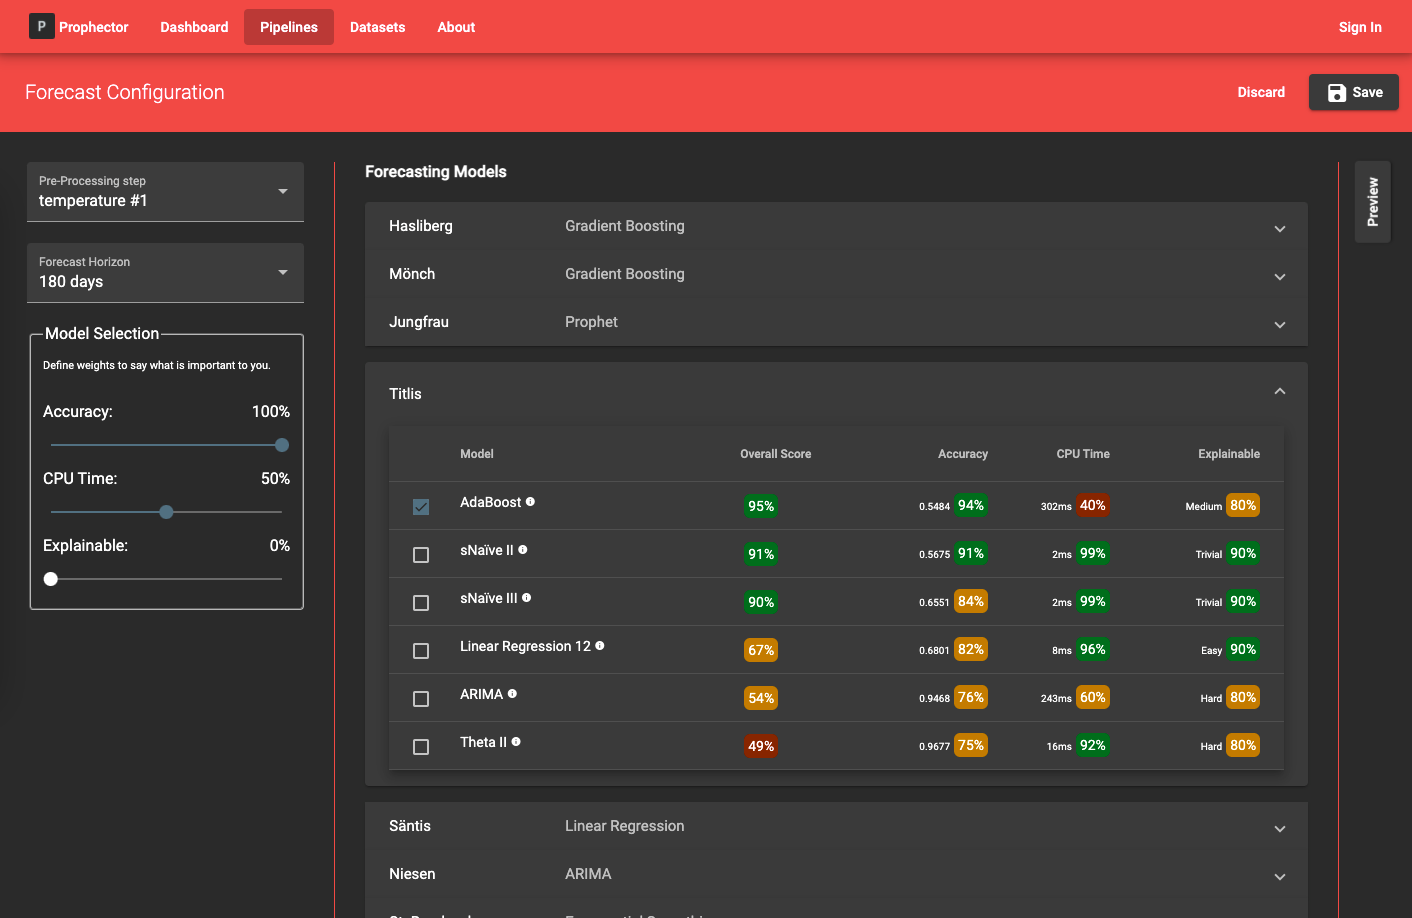
\includegraphics[scale=.3]{Figures/pipeline-config-screenshot.png}}
\caption{The user interface of our application lets users see the timeseries contained in their data source. First they configure sourcing, parsing and pre-processing. Then they reach this screen. Users can change or add multiple pre-processing steps. Based on their forecast horizon and weight sliders, the recommended models change. Each timeseries is presented with a list of possible models with metrics that apply for this type of timeseries. The can manually override the automatic selection. The preview button on the right allows users to inspect forecasts for the first 10 timeseries.}
\label{fig:pipeline-config-screenshot}
\end{figure*}

\subsection{Forecast Analysis}

After the user has configured a pipeline, they can search for timeseries within their dataset. Navigating to this timeseries then reveals the sourced data, the forecast and optionally the anomalies annotated on the graph.

Alongside are meta information such as when this data was fetched, when it was forecasted, the model used, the sensitivity and so forth.

The user commonly wants to act upon seeing the forecast, so it should be easily shareable by URL. If configuration changes become necessary, the in app links should point the user to the configuration of the pipeline steps. If they want to change something particular about this timeseries only, e.g., they want to adjust the anomaly sensitivity for that timeseries, they can do so right there without having to leave the screen..

